\documentclass{paper}

%\usepackage{times}
\usepackage{epsfig}
\usepackage{graphicx}
\usepackage{amsmath}
\usepackage{amssymb}
\usepackage{color}
\usepackage{caption}
\usepackage{subcaption}
\usepackage{here}
\usepackage{todonotes}
\usepackage{titlesec}
\usepackage{here}


% load package with ``framed'' and ``numbered'' option.
%\usepackage[framed,numbered,autolinebreaks,useliterate]{mcode}

% something NOT relevant to the usage of the package.
\setlength{\parindent}{0pt}
\setlength{\parskip}{18pt}

\usepackage[latin1]{inputenc} 
\usepackage[T1]{fontenc} 

\usepackage{listings} 
\lstset{% 
   language=Matlab, 
   basicstyle=\small\ttfamily, 
} 
\graphicspath{{inpainting/Figures/}}

\newcommand{\prox}{\text{prox}}

\title{Image inpainting -- Assignment 2}



\author{Mich\`ele Wyss \\10-104-123}
% //////////////////////////////////////////////////


\begin{document}



\maketitle


% Add figures:
%\begin{figure}[t]
%%\begin{center}
%\quad\quad   \includegraphics[width=1\linewidth]{ass2}
%%\end{center}
%
%\label{fig:performance}
%\end{figure}

\section{Primal-dual formulation}
\label{sec:primal-dual-formulation}
Our objective function that we want to minimize is given by 
$$E(u) = \frac{\lambda}{2} \|u-g\|_\Omega^2 + \|\nabla u\|_2.$$

In General, given an initial problem
$$\min_{x \in X}F(Ku) + G(x),$$
a primal-dual formulation is given by
\begin{equation}
\min_{x \in X} \max_{y \in Y} \langle Kx, y \rangle - F^*(y) + G(x). 
\label{eq:general-primal-dual-formulation}
\end{equation}
In the above formulations, $F$ and $G$ are convex and $K$ is a linear operator. Defining $K = \nabla$, $F = \|\cdot\|_2$ and $G(u) = \frac{\lambda}{2}\|u-g\|_\Omega^2$, we can therefore get the following primal-dual formulation of our original problem:
$$\min_u \max_p \langle p,\nabla u \rangle - F^*(p) + \frac{\lambda}{2} \|u-g\|_\Omega^2,$$
where the Legendre-Fenchel transform of $F$ can easily be found as follows:
\begin{align*}
 F^*(y) = (\|\cdot \|_2)^* (y) &= \sup_x x^Ty - \|x\|_2 \\
 &= \sup_x x^Ty - \max_{\|z\|_2 \leq 1} x^Tz \\
 &= \sup_x \min_{\|z\| \leq 1} x^T (y-z) \\
 &= \begin{cases} 0 ~ \text{if } \|y\| \leq 1, \\ \infty ~ \text{otherwise.} \end{cases}
\end{align*}

\section{Primal-Dual steps}
\label{sec:primal-dual-steps}
Starting again at our general formulation of the saddle-point problem from equation (\ref{eq:general-primal-dual-formulation}), we want to use the following algorithm, proposed by A. Chambolle and T. Pock  (``Algorithm 1'' in \cite{chambolle2011first}):
\begin{align*}
 y^{n+1} &= \prox_{\sigma F^*}(y^n + \sigma K \bar x^n) \\
 x^{n+1} &= \prox_{\tau G}(x^n - \tau K^* y^{n+1}) \\
 \bar x^{n+1} &= x^{n+1} + \theta(x^{n+1} - x^n),
\end{align*}
where $\theta \in (0,1]$ and $\tau \sigma \|K\|^2 < 1.$ 

The operators ``\prox'' \, are so-called \emph{proximity operators}. They are defined as 
\begin{equation}\prox_{\lambda F}(x) := \arg\min_z \frac{1}{2} \|x-z\|_2^2 + \lambda F(z)
\label{eq:def-proximity-operator}
\end{equation}

\subsection{Find $y^{n+1}$}
Finding the proximity operator $\prox_{\sigma (\|\cdot\|)*}$ can be done by e.g. using \emph{Moreau's identity} (sometimes also referred to as \emph{Moreaus's theorem}). This theorem states that
$$\prox_{\lambda F^*}(x) = x - \lambda\, \prox_{\frac{F}{\lambda}}\left(\frac{x}{\lambda}\right).$$

Applying this, we can calculate the proximity operator of the Legendre-Fenchel transform based on the proximity operator of the $l_2$-norm and get
\begin{align*}
 \prox_{\sigma F^*}(y^n + \sigma K \bar x^n) &= y^n + \sigma K \bar x^n - \sigma \, \prox_{\frac{F}{\sigma}}\left(\frac{y^n + \sigma K \bar x^n}{\sigma} \right) \\
 &= (y^n + \sigma K \bar x^n) - \sigma \cdot \frac{y^n + \sigma K \bar x^n}{\sigma} \cdot \max\left\{0, 1 - \frac{1}{\|y^n + \sigma K \bar x^n\|_2}\right\} \\
 &= (y^n + \sigma K \bar x^n) - (y^n + \sigma K \bar x^n) \cdot \max\left\{0, 1 - \frac{1}{\|y^n + \sigma K \bar x^n\|_2}\right\}
\end{align*}
Here, the second equality follows from the fact that $$\prox_{\frac{\|\cdot\|_2}{\sigma}}\left(\frac{x}{\sigma}\right) = \frac{x}{\sigma} \cdot \max\left\{0,1-\frac{1}{\|x\|_2}\right\}.$$
Let's go step by step and consider the two possible cases of how to compute the wanted proximity operator:

\textbf{Case 1: $\|y^n + \sigma K \bar x^n\| \geq 1.$}

In this case we have 
\begin{align*}
 \prox_{\sigma F^*}(y^n + \sigma K \bar x^n) &= (y^n + \sigma K \bar x^n) - (y^n + \sigma K \bar x^n) \cdot \left(1 - \frac{1}{\|y^n + \sigma K \bar x^n\|_2}\right) \\
 &= y^n + \sigma K \bar x^n - (y^n + \sigma K \bar x^n) + \frac{y^n + \sigma K \bar x^n}{\|y^n + \sigma K \bar x^n\|_2} \\
 &= \frac{y^n + \sigma K \bar x^n}{\|y^n + \sigma K \bar x^n\|_2}.
\end{align*}

\textbf{Case 2: $\|y^n + \sigma K \bar x^n\| < 1.$}
\begin{align*}
\prox_{\sigma F^*}(y^n + \sigma K \bar x^n) &=  (y^n + \sigma K \bar x^n) - (y^n + \sigma K \bar x^n) \cdot \max\{0, 1 - \frac{1}{\|y^n + \sigma K \bar x^n\|_2}\} \\
&= (y^n + \sigma K \bar x^n) - (y^n + \sigma K \bar x^n) \cdot 0 \\
&= (y^n + \sigma K \bar x^n).
\end{align*}

Merging the two cases together, we can express the proximity operator in a more compact form:
$$\prox_{\sigma F^*}(y^n + \sigma K \bar x^n) = \frac{y^n + \sigma K \bar x^n}{\max\{1,\|y^n + \sigma K \bar x^n\|_2\}},$$
and remembering that we set $K = \nabla$, we have the following update rule:
\begin{equation}
 y^{n+1} = \frac{y^n + \sigma \nabla \bar x^n}{\max\{1,\|y^n + \sigma \nabla \bar x^n\|_2\}}.
 \label{eq:update-y}
\end{equation}

\subsection{Find $x^{n+1}$}
As opposed to the previous section, we try to find the proximity operator $\prox_{\tau G}(x^n - \tau K^* y^{n+1})$ directly by its definition. Note that $K^*$ is not the Lagrange-Fenchel transform, but simply the \emph{adjoint} operator of $K$. In our case, $K$ is the gradient, and therefore, $K^*$ is the negative of the divergence, $K^* = - \text{div}$. Starting with the definition of a proximity operator given in equation (\ref{eq:def-proximity-operator}), we get 
\begin{align*}
 \prox_{\tau G}(x^n - \tau K^* y^{n+1}) = \arg\min_z \underbrace{\frac{1}{2} \|(x^n - \tau K^* y^{n+1})-z\|_2^2 + \tau \, \frac{\lambda}{2} \, \|z-g\|_\Omega^2}_{=: \tilde E(z)}.
\end{align*}
We try to find the minimum by setting the derivative with respect to $z$ to zero:
\begin{align*}
 \nabla_z \tilde E(z) &= z - (x^n - \tau K^* y^ {n+1}) + \tau \lambda \Omega (z-g) \\
 &= z - x^n + \tau K^* y^{n+1} + \tau \lambda \Omega (z-g) \\
 &= z - x^n + \tau K^* y^{n+1} + \tau \lambda \Omega z -\tau \lambda \Omega g \\
 &= z(1 + \tau \lambda \Omega) - x^n + \tau K^* y^{n+1} - \tau \lambda \Omega g \stackrel{!}{=} 0 \\
 &\Longleftrightarrow z = \frac{x^n - \tau K^* y^{n+1} + \tau \lambda \Omega g}{1 + \tau \lambda \Omega}.
\end{align*}
From this we get the update rule
\begin{equation}x^{n+1} = \frac{x^n + \tau \nabla \cdot y^{n+1} + \tau \lambda \Omega g}{1 + \tau \lambda \Omega},
\label{eq:update-x}
\end{equation}
where $\nabla \cdot y^{n+1}$ denotes the divergence of $y^{n+1}$.

\section{Results}
\subsection{Setting the parameters}
As proposed for the case of a denoising application on p.24 in \cite{chambolle2011first}, I used the value $\tau = 0.01$. It was already mentioned in Section \ref{sec:primal-dual-steps}, that $\tau \sigma \|K\|^2 < 1$ has to be fulfilled. I chose $\sigma = \frac{1}{0.09}$. This ensures that $\tau \sigma \|K\|^2 < 1$ since $\|K\|^2 \leq 8$ (for a proof of this, please consider \cite{chambolle2004algorithm}).
\subsection{Obtained images}
In Figure \ref{fig:results-cat}, there is an example of the obtained results. It's worth mentioning that there's not much of a difference between the image obtained with only $1'000$ iterations and the final output. We can also see that the method already converges very soon from the plot of the objective function $E$ (see Figure \ref{fig:plot-costs}), as opposed to the previously implemented gradient descent method that only converged after up to $10'000$ or even $100'000$ iterations, depending on the learning rate.

\begin{figure}[H]
\centering
\begin{subfigure}[ht]{0.45\textwidth}
	\centering
	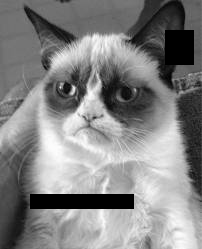
\includegraphics[width=\textwidth]{input-cat}
	\caption*{Input}
\end{subfigure}
~
\begin{subfigure}[ht]{0.45\textwidth}
	\centering
	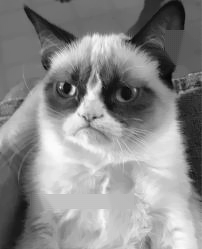
\includegraphics[width=\textwidth]{result-cat-lambda100-theta0_5-iter3000}
	\caption*{Output ($3'000$ iterations)}
\end{subfigure}

\vspace{3mm}
\begin{subfigure}[ht]{0.3\textwidth}
	\centering
	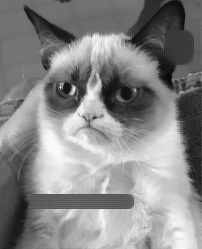
\includegraphics[width=\textwidth]{result-cat-lambda100-theta0_5-iter250}
	\caption*{$250$ iterations}
\end{subfigure}
~
\begin{subfigure}[ht]{0.3\textwidth}
	\centering
	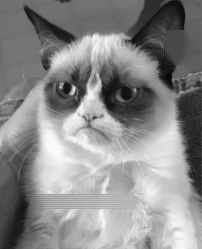
\includegraphics[width=\textwidth]{result-cat-lambda100-theta0_5-iter500}
	\caption*{$500$ iterations}
\end{subfigure}
~
\begin{subfigure}[ht]{0.3\textwidth}
	\centering
	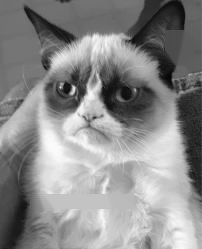
\includegraphics[width=\textwidth]{result-cat-lambda100-theta0_5-iter1000}
	\caption*{$1'000$ iterations}
\end{subfigure}
\caption{The different states of the proceeding of the algorithm. Note that there's not much of a difference between the image obtained with only $1'000$ iterations and the final output. I chose $\theta = 0.5$ and $\lambda = 100$. The other parameters were chosen as mentioned before.}
\label{fig:results-cat}
\end{figure}

\begin{figure}[ht]
 \centering
 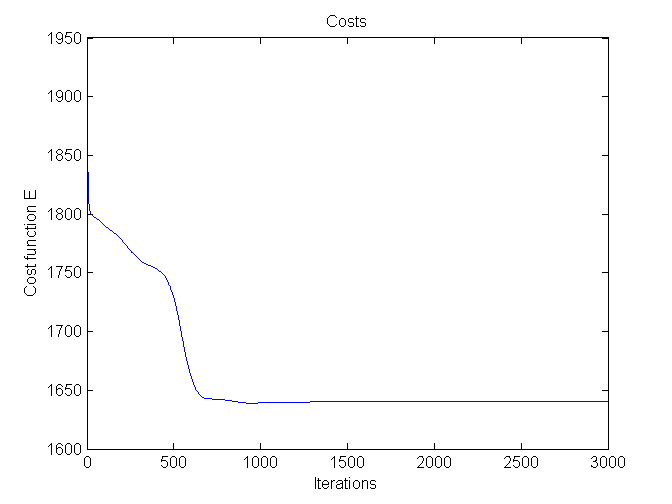
\includegraphics[width=\textwidth]{plot-costs}
  \caption{Plot of the cost function $E$.}
 \label{fig:plot-costs}
\end{figure}


\section{The effect of $\lambda$}
In the objective function
$$E(u) = \frac{\lambda}{2} \|u-g\|_\Omega^2 + \|\nabla u \|_2$$
the parameter $\lambda$ is a \emph{regularization parameter}. It controls the tradeoff between the two constraints of fitting the image and keeping the result smooth. 
A very low $\lambda$, e.g.\ $\lambda = 0.1$ kind of allows the whole image to change. The smoothness contraint is in this case much more important. 
This will make the transitions between the originally available and the inpainted image regions nearly or completely invisible, but the overall image might get significantly oversmoothed. 
A very high $\lambda$-value may fail to end up in a nice-looking smooth image -- in other words, it is likely that there are aprupt changes in the output image. 
Some examples obtained with different values for $\lambda$ are shown in Figure \ref{fig:results-lambda}. Note that $\lambda$ does not heavily influence the number of iterations (as long as the values are not exremely small, the behaviour will stay more or less the same) that is necessary for the algorithm to converge. This was not the case in the gradient descent method, because due to large values it may have been necessary to set a lower learning rate. 

\begin{figure}[ht]
\centering
\begin{subfigure}[ht]{0.3\textwidth}
	\centering
	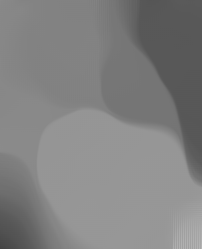
\includegraphics[width=\textwidth]{result-cat-lambda0_1-theta0_5-iter1500}
	\caption*{$\lambda = 0.1$}
\end{subfigure}
~
\begin{subfigure}[ht]{0.3\textwidth}
	\centering
	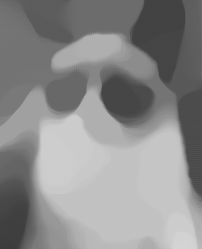
\includegraphics[width=\textwidth]{result-cat-lambda1-theta0_5-iter1500}
	\caption*{$\lambda = 1$}
\end{subfigure}
~
\begin{subfigure}[ht]{0.3\textwidth}
	\centering
	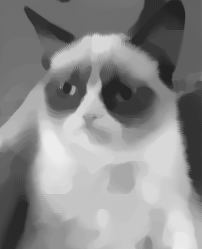
\includegraphics[width=\textwidth]{result-cat-lambda5-theta0_5-iter1500}
	\caption*{$\lambda = 5$}
\end{subfigure}

\vspace{3mm}
\begin{subfigure}[ht]{0.3\textwidth}
	\centering
	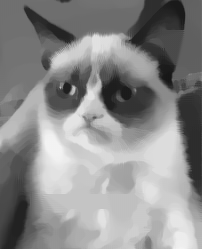
\includegraphics[width=\textwidth]{result-cat-lambda10-theta0_5-iter1500}
	\caption*{$\lambda = 10$}
\end{subfigure}
~
\begin{subfigure}[ht]{0.3\textwidth}
	\centering
	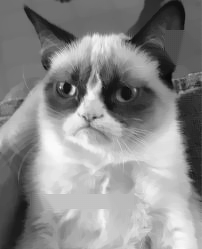
\includegraphics[width=\textwidth]{result-cat-lambda50-theta0_5-iter1500}
	\caption*{$\lambda = 50$}
\end{subfigure}
~
\begin{subfigure}[ht]{0.3\textwidth}
	\centering
	
\includegraphics[width=\textwidth]{result-cat-lambda1000-theta0_5-iter1500}
	\caption*{$\lambda = 1'000$}
\end{subfigure}
\caption{Results with different values for $\lambda$. All the above images were obtained after $1'500$ iterations.}
\label{fig:results-lambda}
\end{figure}

I was not able to find an optimal value for $\lambda$. As can be seen from Figure \ref{fig:plot-ssd}, the higher the value for $\lambda$, the smaller the error gets. However, first of all we see that after reaching a value of $\lambda \approx 100$, the result does not significantly improve with growing $\lambda$-values. Second, it's worth to mention that we can see from the update-rule (\ref{eq:update-x}), that the value of $\lambda$ is in a way meaningless within inpainted regions, since $\Omega$ will be zero in those regions and therefore all the terms containing $\lambda$ will cancel out (however, $\lambda$ of course influences those regions indirectly through the surrounding image content, due to gradients and divergence). This is a possible explanation of why a really huge value for $\lambda$ does not cause very bad results (as it was the case in gradient descent, where a big value could cause the whole algorithm to diverge) -- the image regions that are originally available will be fitted as good as possible, whereas the inpainting regions do not further progress.

However, it is evident that those high values cause some gradient inconsistencies at the borders of the inpainting regions. It might be that the sum of squared distances it not the very best measure to capture this problem.

\begin{figure}[ht]
 \centering
 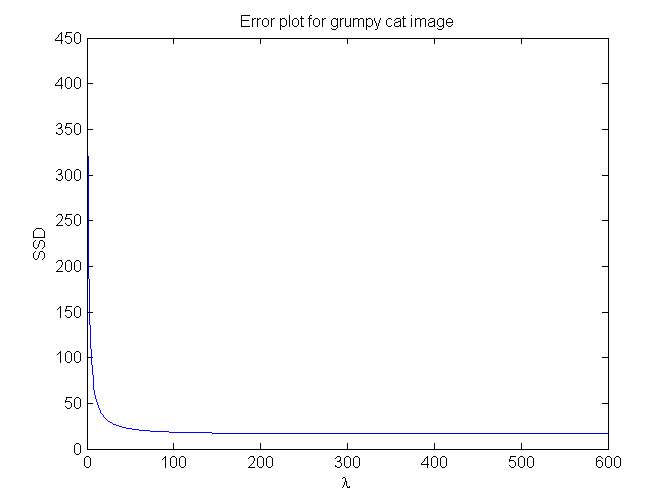
\includegraphics[width=\textwidth]{ssd}
  \caption{$\lambda$ vs. SSD plot. Once $\lambda$ reached the value of $100$, the error is not further reduced in a remarkable way. }
 \label{fig:plot-ssd}
\end{figure}

\section{Conclusions}
Whereas the gradient descent method is simple to implement, it might require a huge amount of iterations and a low learning rate to get to a reasonable result. 
The primal-dual method introduces some additional variables, the dual variables, that made us able to remove coupling of the variable due to the gradient. 
Thanks to that, the method converges remarkably faster than gradient descent, and, moreover, independent from the choice of $\lambda$.

The primal-dual algorithm also contains some tricky aspects like e.g.\ finding useful parameters $\tau$, $\sigma$ and $\theta$. As was also mentioned in \cite{chambolle2011first}, it is not clear how to deal with operators with an unknown norm or even unbounded ones, since the parameters $\tau$ and $\sigma$ do depend on that. The gradient descent method is much simpler to handle since the only thing that may have to be changed is the learning rate (and, possibly, depending on that, the number of iterations).

Also, the theoretical background needed to understand the primal-dual formulations and to understand why the proposed algorithm works, is way more advanced than the theory behind gradient descent, which may make it harder to reason about results and problems.

From the point of view of performance, the two methods are at a comparable level. In my cases, the primal-dual method was able to capture a bit more of the structures, as can be seen in Figure \ref{fig:grad-desc-vs-primal-dual}. This results may not be very representative since in both algorithms the choice of the parameters is probably not the optimal one.

\begin{figure}[ht]
\centering
\begin{subfigure}[ht]{0.45\textwidth}
	\centering
	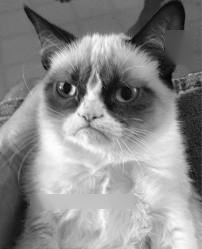
\includegraphics[width=\textwidth]{gradient_descent_cat-iter100000-lambda1000-alpha0_0005}
	\caption*{Gradient descent (SSD = 15.0042) \\100'000 iterations}
\end{subfigure}
~
\begin{subfigure}[ht]{0.45\textwidth}
	\centering
	
\includegraphics[width=\textwidth]{result-cat-lambda1000-theta0_5-iter1500}
	\caption*{Primal-dual (SSD = 16.4611) \\1'500 iterations}
\end{subfigure}
\caption{Comparison between the results obtained with gradient descent and the primal-dual algorithm, both applied with $\lambda = 1'000$. The ear of the cat is visibly more pleasing in the primal-dual result than gradient descent. The SSD to the ground truth, however, is lower with gradient descent.}
\label{fig:grad-desc-vs-primal-dual}
\end{figure}

\bibliographystyle{alphadin}
\nocite{*}

\bibliography{lit}
 \end{document}
 
 